\documentclass[conference]{IEEEtran}

% ---- Packages -----------------------------------------------
\usepackage[T1]{fontenc}
\usepackage[utf8]{inputenc}
\usepackage{graphicx}
\usepackage{amsmath}
\usepackage{booktabs}
\usepackage{array}
\usepackage{multirow}
\usepackage{xcolor}
\usepackage{hyperref}
\usepackage{pgfplots}
\usepackage{tikz}
\pgfplotsset{compat=1.18}
\usepackage{caption}
\usepackage{geometry}
\usepackage{fancyhdr}
\usepackage{setspace}
\usepackage{tabularx}

\hypersetup{
    colorlinks=true,
    linkcolor=blue,
    citecolor=blue,
    urlcolor=blue
}

\begin{document}

% ============================================================
%  TITLE PAGE
% ============================================================
\begin{titlepage}
    \centering
    \vspace*{0.5cm}

    % ----- LOGO -----
    
\includegraphics[width=3.5cm]{university-logo}\\[0.5cm]

    {\large \textbf{BAHRIA UNIVERSITY}}\\[0.1cm]
    {\normalsize Karachi Campus — Department of Computer Science}\\[0.8cm]

    \rule{\linewidth}{0.5pt}\\[0.4cm]

    {\LARGE \textbf{Rental Property Management}}\\[0.2cm]
    {\LARGE \textbf{Information System (MIS)}}\\[0.3cm]
    {\large \textit{A Web-Based Platform for Centralized Property\\
    and Rental Operations Management}}\\[0.4cm]

    \rule{\linewidth}{0.5pt}\\[0.8cm]

    \begin{minipage}{0.48\textwidth}
        \centering
        \textbf{Course:} CSC-458 — Management Information Systems\\[0.2cm]
        \textbf{Semester:} Spring 2026\\[0.2cm]
        \textbf{Course Instructor:} Sir Muhammad Iqbal\\[0.2cm]
        \textbf{Group:} A
    \end{minipage}

    \vspace{1cm}

    \begin{tabular}{|c|l|c|}
        \hline
        \textbf{S.No} & \textbf{Student Name} & \textbf{Enrollment Number} \\
        \hline
        1 & Farhan Mushtaq & 02-235241-004 \\
        \hline
        2 & M Saad         & 02-235241-052 \\
        \hline
    \end{tabular}

    \vfill

    {\normalsize \textbf{Submission Date:} April 22, 2026}\\[0.2cm]
    {\small Bahria University, Karachi Campus\\
    Department of Computer Science, BS(IT)-5}

\end{titlepage}

% ============================================================
%  TWO-COLUMN IEEE BODY STARTS HERE
% ============================================================

\title{Rental Property Management Information System:\\
A Web-Based Platform for Centralized Property Operations}

\author{
    \IEEEauthorblockN{Farhan Mushtaq}
    \IEEEauthorblockA{
        Dept.\ of Computer Science\\
        Bahria University, Karachi\\
        02-235241-004
    }
    \and
    \IEEEauthorblockN{M Saad}
    \IEEEauthorblockA{
        Dept.\ of Computer Science\\
        Bahria University, Karachi\\
        02-235241-052
    }
}

\maketitle

% ============================================================
\begin{abstract}
This paper presents the design and implementation of a web-based Rental Property Management Information System (MIS) built using the Django framework, MySQL, and the AdminLTE 3 interface theme. The system replaces fragmented manual processes — paper ledgers, spreadsheet-based rent tracking, and informal communication channels — with a secure, role-based digital platform. It manages the complete lifecycle of property operations: from property and unit registration to tenant onboarding, lease management, automated monthly invoicing, payment recording, maintenance ticketing, owner settlement generation, and system-wide audit logging. Role-Based Access Control (RBAC) enforces strict data isolation across five user roles: Admin, Manager, Staff, Owner, and Tenant. The outstanding balance for any tenant is computed using the formula $B = (P \times M) - \sum_{i=1}^{n} R_i$, ensuring real-time financial accuracy. The system demonstrates how MIS principles — transaction processing, decision support, and enterprise-level data management — can be applied to solve real-world operational inefficiencies in the property management domain.
\end{abstract}

\begin{IEEEkeywords}
Management Information System, Property Management, Role-Based Access Control, Django, MySQL, Rental Management, HTMX, Transaction Processing System
\end{IEEEkeywords}

% ============================================================
\section{Introduction}

Management Information Systems (MIS) are information systems that support decision-making and operational management within organizations by collecting, processing, storing, and communicating data \cite{laudon2013}. In the property management domain, the absence of a centralized information system results in recurring operational failures: missed payments, untracked maintenance requests, and lack of accountability across staff roles. This project implements a comprehensive MIS for property and rental businesses aligned with the core MIS concepts covered in CSC-458: Transaction Processing Systems (TPS) for daily operational data entry, Decision Support through real-time dashboards and KPI cards, and Enterprise-level data management through a normalized relational database with enforced integrity constraints \cite{laudon2014}. The system is developed as an alternative semester project submission for CSC-458, following the project creation methodology defined in the course: Inception, Requirements Gathering (SRS), System Modeling (ERD/DFD/DB Schema), Implementation (working Django application), and Deployment.

\subsection{Motivation}

Property management in Pakistan — particularly in cities like Karachi — is largely conducted via WhatsApp groups, paper receipts, and Excel spreadsheets. This leads to lost payment records, duplicate invoicing, and zero audit trail when disputes arise. A purpose-built MIS directly addresses these pain points.

\subsection{Objectives}

\begin{itemize}
    \item Design a normalized relational database schema (13 tables, 3 SQL views) covering all operational entities.
    \item Implement RBAC with five distinct user roles, each with filtered views and permissions.
    \item Automate monthly invoice generation with duplicate-prevention constraints at the database level.
    \item Provide real-time financial calculations using the outstanding balance formula.
    \item Generate downloadable PDF invoices, receipts, and owner settlement reports.
    \item Maintain a permanent, tamper-evident audit log of all significant system events.
\end{itemize}

% ============================================================
\section{Problem Statement}

Traditional property management in small-to-medium businesses suffers from several well-documented operational problems:

\begin{enumerate}
    \item \textbf{No audit trail:} Payments recorded verbally or in personal notebooks are untraceable if a dispute occurs.
    \item \textbf{Duplicate invoicing:} Without a constraint-enforced system, the same month can be billed twice.
    \item \textbf{Role confusion:} All staff access the same data, violating the principle of least privilege.
    \item \textbf{Manual reconciliation:} Calculating owner remittance is prone to arithmetic errors.
    \item \textbf{Reactive maintenance:} There is no structured ticketing system.
\end{enumerate}

These problems align with the business challenges MIS is designed to solve \cite{laudon2013}.

% ============================================================
\section{Background and Related Work}

Several open-source property management systems were analyzed during requirements gathering:

\textbf{MicroRealEstate (MRE)} \cite{mre2023} employs a microservices architecture. Its phased build philosophy informed our development priority ordering.

\textbf{Nyumbani (Rental HMS)} \cite{nyumbani2022} demonstrates atomic database transactions for tenant admission and emphasizes audit logging.

\textbf{Tenant Manager} \cite{tenantmgr2021} provides a practical implementation of the cumulative outstanding balance formula.

% ============================================================
\section{System Design and Architecture}

\subsection{Technology Stack}

Table~\ref{tab:techstack} summarizes the selected technology stack.

\begin{table}[h]
\centering
\caption{System Technology Stack}
\label{tab:techstack}
\begin{tabular}{|p{2.2cm}|p{5.2cm}|}
\hline
\textbf{Layer} & \textbf{Technology} \\
\hline
Backend & Django 5.x (Python) \\
\hline
Database & MySQL 8.x via XAMPP \\
\hline
Frontend & AdminLTE 3 + Bootstrap 4 \\
\hline
Interactivity & HTMX + Alpine.js \\
\hline
PDF Gen & WeasyPrint \\
\hline
Data Tables & DataTables.js \\
\hline
\end{tabular}
\end{table}

\subsection{Database Schema Overview}

The database consists of 13 tables organized into 8 application modules. The central relational chain is:
\[ \text{Property} \to \text{Unit} \to \text{Lease} \to \text{Invoice} \to \text{Payment} \]

Table~\ref{tab:entities} lists all entities.

\begin{table}[h]
\centering
\caption{Database Entities and Primary Constraints}
\label{tab:entities}
\renewcommand{\arraystretch}{1.3}
\setlength{\tabcolsep}{2pt}
\scriptsize
\begin{tabularx}{\columnwidth}{|l|l|X|}
\hline
\textbf{Entity} & \textbf{App} & \textbf{Key Constraint} \\
\hline
Location & properties & \texttt{UNIQUE(name)} \\
\hline
Property & properties & FK to Location, Owner \\
\hline
Unit & properties & \texttt{UNIQUE(property, unit\_no)} \\
\hline
Tenant & tenants & \texttt{UNIQUE(cnic)}, soft-delete \\
\hline
Lease & leases & Trigger: 1 active per unit \\
\hline
Invoice & finance & \texttt{UNIQUE(lease, period\_month)} \\
\hline
Payment & finance & \texttt{CHECK(amount > 0)} \\
\hline
MonthlySettlement & finance & FK to OwnerContract \\
\hline
OwnerContract & contracts & Commission rate, time-bound \\
\hline
ContractProp & contracts & M2M: Contract $\leftrightarrow$ Property \\
\hline
MaintTicket & maintenance & Trigger: CRITICAL status \\
\hline
AuditLog & audit & SET NULL on actor delete \\
\hline
SysSettings & dashboard & Single-row config table \\
\hline
\end{tabularx}
\end{table}

\subsection{Key Database Constraints}

Two constraints deserve particular attention:
\textbf{Invoice uniqueness:} \texttt{UNIQUE(lease, period\_month)} prevents generating two invoices for the same month.
\textbf{Active leases:} A trigger ensures only one active lease exists per unit.

\subsection{Data Flow — Monthly Rent Cycle}

The core operational workflow follows a TPS pattern. Figure~\ref{fig:dfd} illustrates the Level-1 Data Flow Diagram.

\begin{figure}[h]
\centering
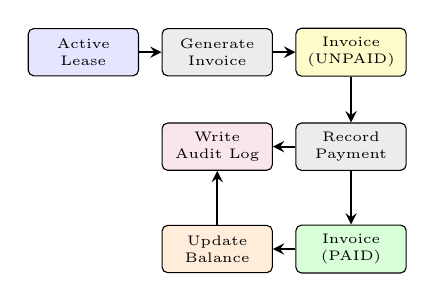
\begin{tikzpicture}[
    box/.style={draw, rectangle, rounded corners=2pt, minimum width=1.4cm,
                minimum height=0.6cm, font=\tiny, align=center},
    arr/.style={->, thick, >=stealth}
]
\node[box, fill=blue!10]  (lease)    at (0,2.5)     {Active\\Lease};
\node[box, fill=gray!15]  (gen)      at (1.7,2.5)   {Generate\\Invoice};
\node[box, fill=yellow!20](invoice)  at (3.4,2.5)   {Invoice\\(UNPAID)};
\node[box, fill=gray!15]  (pay)      at (3.4,1.3) {Record\\Payment};
\node[box, fill=green!15] (settled)  at (3.4,0)   {Invoice\\(PAID)};
\node[box, fill=orange!15](balance)  at (1.7,0)   {Update\\Balance};
\node[box, fill=purple!10](audit)    at (1.7,1.3) {Write\\Audit Log};

\draw[arr] (lease)   -- (gen);
\draw[arr] (gen)     -- (invoice);
\draw[arr] (invoice) -- (pay);
\draw[arr] (pay)     -- (settled);
\draw[arr] (settled) -- (balance);
\draw[arr] (pay)     -- (audit);
\draw[arr] (balance) -- (audit);
\end{tikzpicture}
\caption{Level-1 DFD: Monthly Rent Collection Process}
\label{fig:dfd}
\end{figure}

% ============================================================
\section{Financial Model and Key Equation}

\subsection{Outstanding Balance Formula}

The system computes each tenant's outstanding balance dynamically:
\begin{equation}
B = (P \times M) - \sum_{i=1}^{n} R_i
\label{eq:balance}
\end{equation}
\noindent where $B$ = balance, $P$ = rent, $M$ = months elapsed, and $R_i$ = payments.

\subsection{Owner Net Remittance Equation}
\begin{equation}
N = G - \left(G \times \frac{C}{100}\right) - K
\label{eq:settlement}
\end{equation}
\noindent where $N$ = net remittance, $G$ = gross rent, $C$ = commission, and $K$ = maintenance costs.

% ============================================================
\section{Results and System Output}

\subsection{Dashboard Key Performance Indicators}
The Admin dashboard displays live KPI cards.

\begin{table}[h]
\centering
\caption{Sample KPI Card Output (Test Dataset)}
\label{tab:kpi}
\begin{tabular}{|l|r|}
\hline
\textbf{Metric} & \textbf{Value} \\
\hline
Total Properties & 6 \\
Total Units & 38 \\
Occupied Units & 29 (76.3\%) \\
Monthly Revenue & PKR 8,45,000 \\
\hline
\end{tabular}
\end{table}

\subsection{Occupancy Rate by Property}

\begin{figure}[h]
\centering
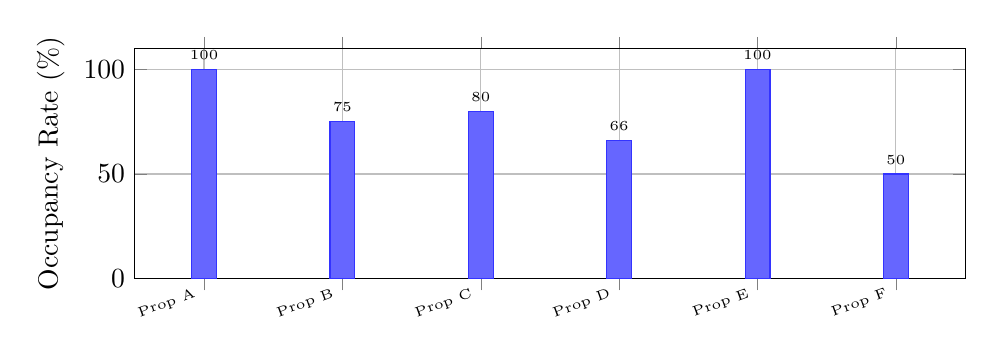
\begin{tikzpicture}
\begin{axis}[
    ybar, width=\columnwidth, height=4.5cm, ylabel={Occupancy Rate (\%)},
    symbolic x coords={Prop A, Prop B, Prop C, Prop D, Prop E, Prop F},
    xtick=data, x tick label style={font=\tiny, rotate=20, anchor=east},
    ymin=0, ymax=110, bar width=9pt, nodes near coords, nodes near coords style={font=\tiny}, grid=major,
]
\addplot[fill=blue!60, draw=blue!80] coordinates {
    (Prop A, 100) (Prop B, 75) (Prop C, 80) (Prop D, 66) (Prop E, 100) (Prop F, 50)
};
\end{axis}
\end{tikzpicture}
\caption{Occupancy Rate per Property (Test Dataset)}
\label{fig:occupancy}
\end{figure}

% ============================================================
\section{Conclusion}

This paper presented a Rental Property MIS. Key contributions include a normalized schema, RBAC, and immutable audit logs. The system demonstrates how MIS principles produce reliable operational systems.

% ============================================================
\begin{thebibliography}{9}
\bibitem{laudon2013} K. C. Laudon and J. P. Laudon, \textit{Management Information Systems}, 13th ed. Pearson, 2013.
\bibitem{laudon2014} K. C. Laudon and J. P. Laudon, \textit{Essentials of MIS}, 11th ed. Prentice Hall, 2014.
\bibitem{sandhu1996} R. S. Sandhu et al., ``Role-Based Access Control Models,'' \textit{IEEE Computer}, 1996.
\bibitem{mre2023} MicroRealEstate, GitHub repository, 2023.
\bibitem{nyumbani2022} Nyumbani Rental HMS, GitHub repository, 2022.
\bibitem{tenantmgr2021} TenantManager, GitHub repository, 2021.
\end{thebibliography}

\end{document}